\documentclass[12pt]{article}
\usepackage{microtype}

% The preceding line is only needed to identify funding in the first footnote. If that is unneeded, please comment it out.
\usepackage{amsmath,amssymb,amsfonts}
\usepackage{algorithmic}
\usepackage{graphicx}
\usepackage{textcomp}
\usepackage{xcolor}
\usepackage{url}
\usepackage{listings}
\usepackage{courier}
\usepackage{xspace}
\usepackage{multirow}
\usepackage{colortbl}
\usepackage{blindtext}
\usepackage{float}
\usepackage{hyperref}
%\usepackage[font=scriptsize]{caption}
%\newcommand{\sd}[1]{\textbf{"\textsc{SD:}} \textit{#1}"}
%Dessin
\usepackage{tikz}
\usepackage{verbatim}
\usepackage{graphicx}
\usepackage[utf8]{inputenc}
\usepackage[english]{babel}
\usepackage{subfigure}
 \newboolean{showcomments}
\setboolean{showcomments}{true}
\ifthenelse{\boolean{showcomments}}
  {\newcommand{\bnote}[2]{
	\fbox{\bfseries\sffamily\scriptsize#1}
    {\sf\small$\blacktriangleright$\textit{#2}$\blacktriangleleft$}
    % \marginpar{\fbox{\bfseries\sffamily#1}}
   }
   \newcommand{\cvsversion}{\emph{\scriptsize$-$Id: macros.tex,v 1.1.1.1 2007/02/28 13:43:36 bergel Exp $-$}}
  }
  {\newcommand{\bnote}[2]{}
   \newcommand{\cvsversion}{}
  } 


\newcommand{\here}{\bnote{***}{CONTINUE HERE}}
\newcommand{\nb}[1]{\bnote{NB}{#1}}

\newcommand{\fix}[1]{\bnote{FIX}{#1}}
%%%% add your own macros 


\newcommand{\an}[1]{\bnote{Anne}{#1}}
\newcommand{\sd}[1]{\bnote{Stef}{#1}}
\newcommand{\ja}[1]{\bnote{Jannik}{#1}}
\newcommand{\md}[1]{\bnote{MD}{#1}}
\newcommand{\caro}[1]{\bnote{Caro}{#1}}
\newcommand{\jr}[1]{\bnote{JRe}{#1}}
\newcommand{\lf}[1]{\bnote{Luc}{#1}}
\newcommand{\gp}[1]{\bnote{Guille}{#1}}
\newcommand{\pt}[1]{\bnote{Pablo}{#1}}
\newcommand{\theo}[1]{\bnote{Theo}{#1}}
\newcommand{\spb}[1]{\bnote{Santiago}{#1}}
\newcommand{\bv}[1]{\bnote{Beno\^{i}t}{#1}}

\graphicspath{{figures/}}
%%% 


\newcommand{\figref}[1]{Figure~\ref{fig:#1}}
\newcommand{\figlabel}[1]{\label{fig:#1}}
\newcommand{\tabref}[1]{Table~\ref{tab:#1}}
\newcommand{\layout}[1]{#1}
\newcommand{\commented}[1]{}
\newcommand{\secref}[1]{Section \ref{sec:#1}}
\newcommand{\seclabel}[1]{\label{sec:#1}}

%\newcommand{\ct}[1]{\textsf{#1}}
\newcommand{\stCode}[1]{\textsf{#1}}
\newcommand{\stMethod}[1]{\textsf{#1}}
\newcommand{\sep}{\texttt{>>}\xspace}
\newcommand{\stAssoc}{\texttt{->}\xspace}

\newcommand{\stBar}{$\mid$}
\newcommand{\stSelector}{$\gg$}
\newcommand{\ret}{\^{}}
\newcommand{\msup}{$>$}
%\newcommand{\ret}{$\uparrow$\xspace}

\newcommand{\myparagraph}[1]{\noindent\textbf{#1.}}
\newcommand{\eg}{\emph{e.g.,}\xspace}
\newcommand{\ie}{\emph{i.e.,}\xspace}
\newcommand{\etal}{\emph{et al.,}\xspace}
\newcommand{\ct}[1]{{\textsf{#1}}\xspace}


\newenvironment{code}
    {\begin{alltt}\sffamily}
    {\end{alltt}\normalsize}

\newcommand{\defaultScale}{0.55}
\newcommand{\pic}[3]{
   \begin{figure}[h]
   \begin{center}
   \includegraphics[scale=\defaultScale]{#1}
   \caption{#2}
   \label{#3}
   \end{center}
   \end{figure}
}

\newcommand{\twocolumnpic}[3]{
   \begin{figure*}[!ht]
   \begin{center}
   \includegraphics[scale=\defaultScale]{#1}
   \caption{#2}
   \label{#3}
   \end{center}
   \end{figure*}}

\newcommand{\infe}{$<$}
\newcommand{\supe}{$\rightarrow$\xspace}
\newcommand{\di}{$\gg$\xspace}
\newcommand{\adhoc}{\textit{ad-hoc}\xspace}

\usepackage{url}            
\makeatletter
\def\url@leostyle{%
  \@ifundefined{selectfont}{\def\UrlFont{\sf}}{\def\UrlFont{\small\sffamily}}}
\makeatother
% Now actually use the newly defined style.
\urlstyle{leo}




 
\author{
        Bragagnolo Santiago, Ferlicot Cyril
}
\title{Projet GIS - Anti-monopoly}
\date{\today}

 
\begin{document}
\maketitle
\emph{Cet exercise est basé sur un exercice proposé dans le cour de Paradigmes de programmation, à l'UTN, Argentine.}

\section{Introduction}

\begin{figure}
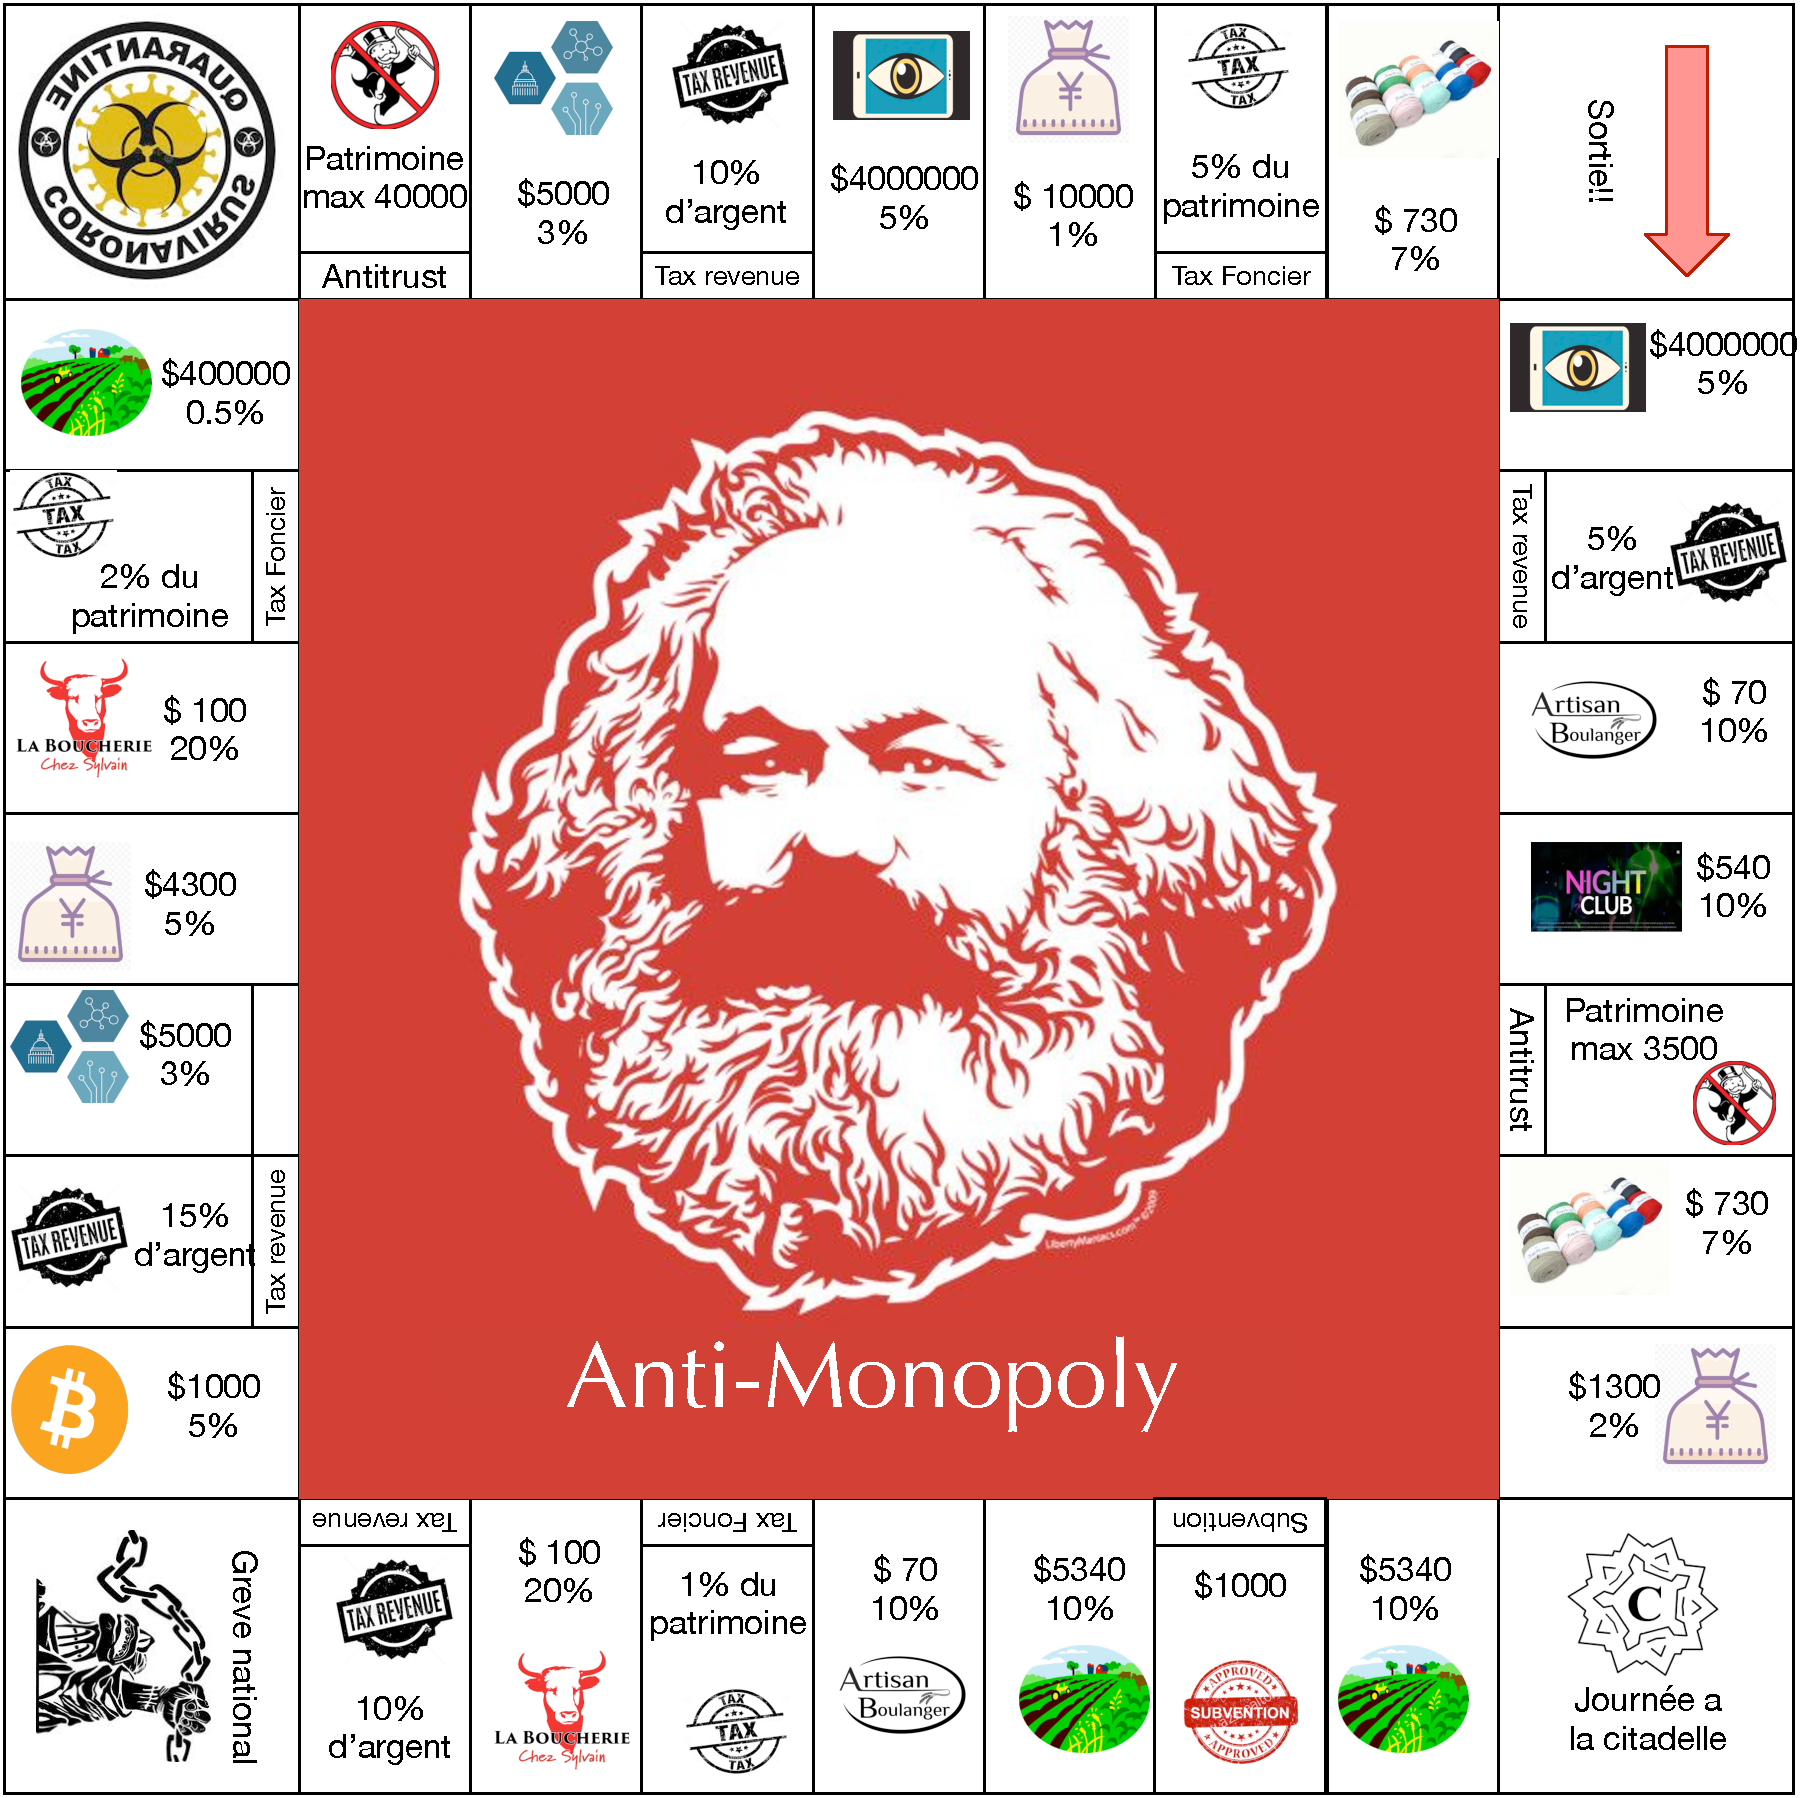
\includegraphics[width=15cm,height=15cm,keepaspectratio]{figures/board.pdf}
\caption{Exemple de tableau de jeu}
\label{fig:tableau}
\end{figure}

	Vous souhaitez implémenter la simulation d'un jeu du style \emph{Monopoly} dans lequel les joueurs cherchent
à augmenter leur patrimoine en marchant sur un chemin où ils doivent prendre des décisions 
d'investissement et faire certaines actions. Attention toutefois à ne pas trop investir, car 
les lois antitrust peuvent vous obliger à distribuer votre richesse.


\section{Caractéristiques du jeu}

    \subsection{Le plateau du jeu}
    Le \textbf{plateau} est constitué d'un chemin circulaire composé de \textbf{cases},
dans chacune desquelles il y a des indications. Une case marquée \textbf{sortie}
indique le point de départ du jeu.
Vous pourrez utiliser la configuration présentée dans l'image \autoref{fig:tableau}, ou inventer de nouvelles configurations par vous même. 
Le but n'est pas de réussir à construire un plateau équilibré, mais d'avoir suffisamment des cases pour pouvoir simuler le jeu et couvrir tous les cas demandés.
	
    \subsection{Les joueurs}
   
    Il peut y avoir autant de \textbf{joueurs} que souhaité. Chaque joueur a un
montant d'argent initial. Au fur et à mesure que le jeu progresse, chacun des joueurs accroit
ou décroit son argent, selon les décisions d'investissement qu'ils prennent ou d'autres
circonstances. Les capitaux propres d'un joueur correspondent à
son argent plus l'évaluation de tous les investissements qu'il possède.
Si un joueur perd tous ses capitaux il a perdu: il ne peut pas continuer à jouer.
    
    \subsection{L'\'Etat}
    
    L'\'Etat est un acteur social dont la fonction principale est de réguler l'activité économique des
différents joueurs. Il possède des ressources financières. L'État ne participe pas
au jeu en marchant sur le plateau, mais interagit avec tous les joueurs comme expliqué plus bas.

    \subsection{La dynamique de jeu}
    
    Initialement, tous les joueurs sont placés dans la case \textbf{sortie}. 

À tour de rôle, chacun lance un \textbf{dé} et avance d'où il se trouve d'autant de cases que l'indique le dé. 
Le joueur doit ensuite suivre les instructions indiquées dans la case et prend les décisions économiques qu'il juge appropriées.
    
De cette manière, tous les joueurs avancent au travers du plateau et font leur stratégie. 
Comme l'itinéraire est circulaire, il n'y a pas de point d'arrivée prédéterminé,
raison pour laquelle ils continuent à tourner jusqu'à la fin du jeu. 
Le jeu se termine s'il ne reste qu'un seul joueur, si l'État échoue ou si l'on souhaite mettre fin au jeu.
Pour cette simulation, la personne pouvant décider de mettre fin au jeu est le spectateur lui même.

    
    \subsection{Les cases}
  
    	Comme on peut voir dans la \autoref{fig:cases}, il existe dans ce jeu différent type de cases. Voici leur particularités:
    \begin{itemize}
        \item \textbf{Investissement}: L'investissement est une case qui rapporte des bénéfices à son propriétaire.
        	Chaque investissement est caractérisé par une valeur nominal et un pourcentage qui représente le bénéfice que cet investissement rapporte. 
		L'investissement a deux états possibles: disponible, et approprié.
		Quand un joueur arrive sur cet case, ses actions possibles dépendent de l'état de l'investissement.
		Si l'investissement est possédé par un autre joueur, le joueur arrivant doit payer à son propriétaire l'utilité de cet investissement.
		Par contre, si l'investissement est disponible, le joueur peut décider de l'acheter ou de le laissez passer. \footnote{ Plus de détailles sur les investissements dans la prochaine section }
		
	
        \item \textbf{Loi antitrust}: Oblige le joueur à céder assez d'investissement pour que la valeur de ses propriétés soit sous le seuil maximum fixé par l'État. 
    Ces investissements reviennent à l'État qui paie le joueur la moitié de leur prix d'achat. 

    Par exemple, si le maximal d'investissements est 500000 euros, et un joueur ayant 3 investissements de 200000 (soit un total de 600000), doit laisser partir un investissement.  
    Dans la même configuration, si un joueur ayant 3 investissements de 300000 (soit un total de 900000), il doit céder deux investissements. 
    Une fois entre les mains de l'état, ces investissements deviennent de nouveau disponibles.

        \item  \textbf{Bureau Finances publiques}: Oblige le joueur à payer à l'État un pourcentage de ses
    capitaux propres, s'ils dépasseraient une certaine valeur. Chaque taxe se calcule comme un pourcentage du patrimoine du joueur.
    La seule différence entre les types d'impôts, hors leur nom, est le pourcentage de prélèvement. 
    Par exemples: un impôt sur le revenu de 25\% du patrimoine, un impôt foncier de 10\% du patrimoine, etc.
        \item \textbf{Subvention}: Le joueur reçoit de l'État le montant indiqué dans la case.
        \item \textbf{Repos}: C'est une case vide dans laquelle rien ne se passe. La \textbf{sortie} en fait partie.
    \end{itemize}
    
    
	  \begin{figure}
    \centering
    \subfigure[]{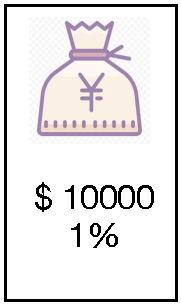
\includegraphics[width=2cm,height=2cm,keepaspectratio]{figures/investissement.pdf}} 
    \subfigure[]{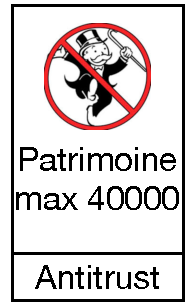
\includegraphics[width=2cm,height=2cm,keepaspectratio]{figures/antitrust.pdf}} 
    \subfigure[]{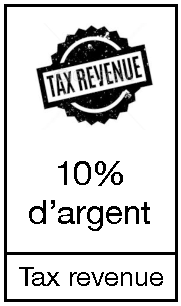
\includegraphics[width=2cm,height=2cm,keepaspectratio]{figures/taxe.pdf}}
       \subfigure[]{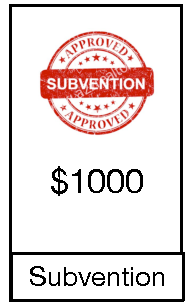
\includegraphics[width=2cm,height=2cm,keepaspectratio]{figures/subvention.pdf}}
      \subfigure[]{
\includegraphics[width=2cm,height=2cm,keepaspectratio]{figures/rienfaire.pdf}}

   
    \caption{(a) Investissment (b) Loi antitrust (c) Finances publiques (d) Subvention (e) Activite non comercial}
    \label{fig:cases}
\end{figure}

    \subsection{Investissements}
	Les \textbf{investissements} sont le principal moyen pour les joueurs de gagner de l'argent. 
	Initialement L'\'Etat les possède tous.
	Lorsqu'un investissement est possédé par l'état, on le considère \textbf{disponible} à l'achat. 
	Par contre, si un investissement est possédé par un joueur, on le considère \textbf{approprié}.
	
	Chaque investissement a un prix de référence (la valeur nominal),  et un pourcentage de bénéfice.
	
	Lorsqu'un joueur tombe sur une case investissement disponible, il peut décider de l'acheter. 
	Pour ce, il doit payer à l'état la valeur nominal de l'investissement. 
	
	Lorsqu'un joueur tombe sur une case investissement approprié, il doit payer au propriétaire la valeur d'utilité ce cet investissement. 
	La valeur d'utilité est correspond au pourcentage de bénéfice de l'investissement de son prix d'achat. 
	
	Par exemple: Un joueur tombant sur un investissement approprié de 10000e à 1\% devra payer 100e au joueur le possédant.
	 
	
    \subsection{Style des joueurs}
    S'agissant d'une simulation, où les décisions de joueurs sont prises par le programme, on doit définir des profiles de joueurs.
    Les profiles proposés sont: \textbf{agressif} et \textbf{prudent}.
    
   Chaque type de joueur prendra des décisions différemment.
   
   \paragraph {Le joueur Agressif}  va essayer de tout prendre le plus vite possible. 
   \begin{itemize}
   	\item En rapport aux investissements: S'il a suffisamment l'argent, il achète tous les investissements possibles.
	\item En rapport aux loi antitrust: Au moment de choisir quels investissements se faire exproprier, il choisi les moins chers.
   \end{itemize}
   
  
   \paragraph {Le joueur Prudent}  va prendre des décisions plus informées . 
    \begin{itemize}
   	\item En rapport aux investissements: Il ne prendra jamais plus qu'une quantité maximale d'investissements (Cette valeur est configurable). De plus, il n'achètera rien de plus cher que 20\% de ses capitaux. 
	\item En rapport aux loi antitrust: Au moment de choisir quel investissement se faire exproprier, il choisi les plus chers.
   \end{itemize}


\section{Simulation}

 La simulation de ce jeu comprend trois phases:
 \begin{description} 
 	\item [Configuration:] L'utilisateur configure la simulation
	\item [Jeu:] Le jeu démarre. 
	\item [Communication des résultats:] On communique les résultats du jeu  
\end{description}
 
 
 \paragraph{La configuration} Il s'agit du moment où le joueur doit exprimer quel type de simulation il souhaite. 
	Dans une console interactive, on laisse  l'utilisateur définir la quantité des joueurs pour chaque type (Agressif / Prudent), le capital des joueurs au départ, le capital de l'État et le profil de simulation. 
 
  Chaque profil de simulation définie quel tableau utiliser, comment partager l'argent entre les joueurs, les pourcentages d'impôts, l'argent minimal pour payer impôts , les pourcentages d'utilité des investissements et le patrimoine maximale pour la loi antitrust à appliquer. 
  Le joueur doit être capable de choisir entre au moins deux des profils suivants: 
  \begin{itemize}
  	\item \textbf{NeoLiberal}~: Certains joueurs ont beaucoup d'argent et d'autres en ont peu. L'état défini des mesures antitrust légères.
  	\item \textbf{Socialiste}~: Tous les joueurs ont autant d'argent au départ. L'état fixe beaucoup de taxes.
  	\item \textbf{Capitaliste}~: Tous les joueurs sont agressifs, les pourcentages de profits sont élevés,  les pourcentage d'investissement sont plus élevés.
  	\item \textbf{Progressiste} : Se joue avec plus de joueurs, les lois antitrust sont strictes et combinées avec des subventions élevées, les pourcentages de profits sont modérés.
  	\item \textbf{l'Europe après le Covid-19} : (au choix de chacun).
\end{itemize}
 
 
  \paragraph{Le jeu}. 
  	Une fois que l'on à fourni toute les informations, ont fait jouer les joueurs à tour de rôle.
	
	 En utilisent une génération de numéros aléatoires pour représenter le dé, on fait jouer chaque joueur et on informe ce qu'il a fait.
	 
	 Une fois que le tour est fini (tous les joueurs ont joués) on vérifie si le jeu est fini. S'il l'est, on saute à la dernière phase. 
	 
	 Si le jeu n'est pas finit, on demande à l'utilisateur s'il veut continuer la simulation. Si oui, on procède au suivant tour de rôle, sinon, on saute à la dernière phase.
	
  
  \paragraph{La Communication des résultats} Informe de la raison du fin de jeu, déclare quel joueur à gagné la partie, imprime le classement des joueurs et l'impression l'état de l'État. 
  	Par exemple
\begingroup\makeatletter\def\@currenvir{verbatim}
\verbatim
	  L'État à échoue! 
	
	  Gagnant: Joueur 1 
	  ================
	  	
	   #     Nom            Investissements   Liquide     Patrimoine
	   1 -   Joueur 1       6000              1010        7010
	   1 -   Joueur 2       6000              1010        7010
	   1 -   Joueur 3       6000              1010        7010
	   ==================================================
   État - 
        Investissements: 0
        Liquide: 0
\end{verbatim}
   


        
\section{Exigences du projet}

	L'implémentation demandée suivra ces jalons de livraison:
	
	\begin{description}
		\item [Lundi 1/Juin - 5 Points ] Livraison d'une conception pour répondre aux contraintes de l'exercice.
		\item [A livrer à la fin de chaque cours - 3 Points ] Les développements du cours comprenant au moins 1 test unitaire utile par cours.
		\item [Lundi 8/Juin - 2 Points] Livraison de l'implémentation de la création du plateau.
		\item [Vendredi 19/Juin - 5 Points]  Livraison d'une révision de la conception UML suite à l'implémentation et d'un court rapport expliquant les raisons de l'évolution de l'UML s'il y en a eu plus implémentation complète de la simulation. 
	\end{description} 
	
	
	\paragraph{Conception} 
		La conception du projet s'agit d'une proposition conceptuelle de solution pour répondre a l'exercice. 
		Est attendu un modèle UML des classes, l'implémentation en pseudo code de la fonction de simulation d'un tour de rôle, et un rapport de conception qui explique le choix des entité, des types structurel (List, Arrays, etc) et qui propose des fonctionnalités importante à tester unitairement, en expliquent la raison de leurs importance.
		
	\paragraph{Implémentation de la création du plateau}
		Ceci est le premier point formel du travail.  Est attendu le code nécessaire à la création d'un plateau de jeu et son utilisation. 
		Ce point ce fait en accord avec le tuteur.
		
	\paragraph{Tests}
		Les tests unitaires sont un des points les plus importants dans le développement moderne. Ils sont indispensables pour le bon développement d'un projet et sont incontournables pour les professionnels.
		À là fin de chaque jour de travail, il est attendu l'ajout au minima d'un test unitaire.
		Le test sera joint d'une explication sous forme de commentaire de méthode comprenant: Qu'est ce qui est testé ? Quels risques le code à tester présentent ? Comment le teste réduit ce danger ?.
		À la fin de chaque jour, le tuteur vas regardé le travail fourni dans votre dépôt github pour chercher ce test. Vous pouvez aider votre tuteur en indiquent la localisation sur Discord. 
		
	\paragraph{Conception partie deux }
		La deuxième partie de la conception s'agit d'un analyse entre la proposition initiale et la réalité . 
		Est attendu dans un rapport une réflexion sur les décisions de modifications prises, comment elles ont affectées le modèle et le travail et ce qui pourrait être fait pour faire mieux pour un futur projet. 
		Cet livrable comprendra un diagramme UML de l'implémentation finale (qui doit être très fidèle au code) et le rapport. 
	
	\paragraph{L'implémentation}
		Le dernier cours servira à présenter l'implémentation finale du projet. Chaque groupe présentera via partagera d'écran une démonstration en direct du fonctionnement de leur projet et expliquera en 2 minutes les challenges les plus importantes qu'ils ont rencontrés. 
		Cette présentation se fera en face des autres groupes pour que tout le monde puisse observer chaque projet et comprendre les différences et similitudes. 
		Dans un second temps, chaque groupe aura une discussion privée avec leur tuteur au cours de laquelle celui-ci pourra poser des questions.
			
	
	
	\section{Bonus}
	
	Le cours est noté sur 20 points. 
	Si vous terminez en avance, il est possible de demander des fonctionnalités supplémentaires à implémenter. Ceci peut rapporter jusqu'à deux points bonus. (Le maximum restant 20 points. Si la note sans bonus est supérieure à 18, elle ne pourra pas dépasser les 20).
	
\end{document}

